\documentclass[12pt]{article}
\usepackage{a4wide}
\usepackage[utf8]{inputenc}
\usepackage[T1]{fontenc}
\usepackage{hyperref}
\usepackage{algorithm,algpseudocode}
\usepackage{float}
\usepackage{amsmath} 
\usepackage{amssymb} 
\usepackage{graphicx}
\graphicspath{{figures/}}          % pipeline writes PDFs/PNGs here
\usepackage{subcaption}
\usepackage{booktabs}
\usepackage{tabularx}
\usepackage{multirow}
\usepackage{listings}
\lstset{basicstyle=\ttfamily\small, breaklines=true, frame=single,
        numbers=left, numberstyle=\tiny}
\usepackage{lineno}
\usepackage{setspace}
\onehalfspacing
\title{rdf-solve: Interoperable RDF for the Life Sciences through Automated Schema Mining and Semantic Mappings}
\author{Javier Millan Acosta \and Egon Willighagen \and More}                           % Will see
\date{\today}

\begin{document}

\maketitle
\linenumbers

\begin{abstract}

The life sciences community has produced many RDF knowledge bases encoding
decades of curated biological data, collectively forming the Life Sciences
Linked Open Data (LSLOD) cloud.
RDF allows domains such as chemistry, agriculture, and disease research to
define or reuse vocabularies, properties, and class hierarchies as schemas for
their typed statements, but this flexibility fragments representation: for instance,
the same aminoacid sequence may be modeled differently across datasets depending on
whether it is treated as a sequence, a structure, or a pathway component.
Schemas are usually documented in publications rather than as linked data, so
finding which classes and properties exist across resources remains largely
manual and must be repeated when databases are updated.
Prior meta-analyses estimated vocabulary reuse at under 20\,\% and concluded
the cloud is less connected than assumed, yet their analyses remain descriptive:
latent overlap is identified statistically but no integration bridges are
constructed and no machine-readable schema artefacts are produced.

We describe a three-stage methodology.
First, co-occurrence patterns are mined automatically from SPARQL endpoints to
approximate database schemas, against locally deployed endpoints when data dumps
are available or against remote endpoints directly, and serialized in widely
adopted formats with full provenance metadata.
Second, a mapping layer is constructed from instance-based URI probing and
curated mapping sets, linking classes and properties across resources.
Third, inference over the combined mapping graph materializes bridges via
transitivity and inversion, yielding a connectivity graph that makes explicit
which dataset pairs share compatible schema elements and can be concretely
joined.

The methodology is implemented in rdf-solve and applied to N LSLOD datasets,
recovering implicit schema structure and publishing it as machine-readable
linked data and graph and relational exports, lowering the barrier for
federated querying, data integration, and longitudinal schema monitoring.

\end{abstract}

\end{abstract}


\section{Introduction}

\subsection{Knowledge representation in the life sciences}

Knowledge bases (...). \cite{guarino_ontologies_nodate}


The Resource Description Framework (RDF) models information as subject--predicate--object
triples whose nodes are identified by Uniform Resource Identifiers
(URIs)~\cite{specifications}.
RDF Schema (RDFS) and the Web Ontology Language (OWL) layer class hierarchies,
property constraints, and logical definitions on top of this
model~\cite{goodsources}.
The biomedical community was among the earliest adopters of Semantic Web
technologies for knowledge management and clinical decision
support~\cite{goodsources}, and the resulting Life Sciences Linked Open Data
(LSLOD) cloud now spans %howmany% 
RDF resources~\cite{kamdar_empirical_2021}.

RDF offers several structural advantages for large-scale data integration.
Its uniform syntax and schema-less flexibility support federated querying
across multiple heterogeneous sources with minimal syntactic
adaptation~\cite{goodsources}.
The use of URIs also makes resources web-dereferenceable: each entity can
be looked up via standard HTTP ~\cite{antoniou_zero-knowledge_2011}.
Semantics encoded in RDFS and OWL enable software reasoners to verify
consistency and generate novel inferences from existing
assertions~\cite{goodsources}, and the linking model facilitates discovery of
related resources even when underlying schemas differ~\cite{goodsources}.
                                                % Thapa & Giese — add bib key when available

\subsection{The gap}

Despite these properties, the LSLOD cloud faces significant
interoperability challenges.
There is semantic heterogeneity due to varying entity
notations, diverse schemas, and a insufficient common vocabulary
reuse~\cite{kamdar_empirical_2021}.
%"To the point where..." %decide phrasing, without mappings between equivalent entities, the question of to which point these datasets can truly be considered linked ~\cite{goodsources}.
Analyzing complex knowledge graphs requires extensive computational skills
and deep knowledge of domain-specific terminologies~\cite{goodsources}, and researchers often struggle to
find sources available and accessible on the Web~\cite{goodsources}.
Recent work on zero-shot SPARQL generation shows that even LLM agents must
probe endpoint schemas interactively before they can construct correct
queries~\cite{walter_grasp_2025}, which points at the practical importance of
discoverable, machine-readable schema information. % Missing here: Expasy paper SPARQL-LLM!!
Neural machine translation approaches to SPARQL face a related bottleneck:
generating correct queries for rare or unseen URIs (the out-of-vocabulary
problem) remains difficult without a machine-readable schema to ground
generation~\cite{goodsources}.                                               % Reyd et al. — add bib key when available

Knowing which ontologies a dataset imports does not reveal its actual
structure: which classes are instantiated, which entailments appear,
how often a property appears, or where values are missing cannot be inferred from ontology declarations
alone.

This is why wo datasets that (partially) reuse the same ontology can have very different practical
shapes while two datasets with disjoint vocabularies can have overlapping
patterns that remain invisible without mappings.
A meta-analysis of approximately 80 LSLOD sources estimated vocabulary
reuse at under 20\,\% and concluded that the cloud "is not actually as
densely connected as is often
indicated"~\cite{kamdar_empirical_2021}.

A further conceptual barrier stems from the evolution of schema
philosophies.
The Semantic Web community has traditionally treated schemas as
\emph{descriptive}; promoting flexibility; while the database community
regards them as \emph{prescriptive}; enforcing
validation~\cite{ahmetaj_common_2025}.
The development of validation languages such as SHACL and
ShEx~\cite{ahmetaj_common_2025,mihindukulasooriya_rdf_2018} % add their specifications and original citations!
reflects a convergence of these
views.

RDF datasets attempt to reuse standard terms but often represent them with
different notations or namespaces; e.g., varying URI patterns for the
same ChEBI identifier; which technically prevents automated federation
and integration\cite{hoyt_unifying_2022, its sources too}.

\cite{maillot_eat_2025} read maillot.

\subsection{Related work}

\paragraph*{Linked data profiling and RDF shape induction.}
Several profiling systems extract structural summaries from SPARQL
endpoints.
Loupe~\cite{loupe2015} mines class, property, and triple-pattern
statistics and presents them through an interactive web interface.
ABSTAT~\cite{abstat2016} computes ontology-driven linked data summaries
with pattern minimization.
ProLOD~\cite{prolod2010} profiles linked open data using statistical
and structural analysis.

Mihindukulasooriya et~al.~\cite{mihindukulasooriya_rdf_2018} use machine
learning; specifically Random Forest classifiers trained on profiled
RDF data from Loupe; to automatically induce integrity constraints in
SHACL and ShEx, achieving up to 97\,\% precision in cardinality
estimation.
Several methods have been developed to analyze and characterize RDF data,
each addressing a distinct slice of the schema discoverability problem.
IndeGx \cite{maillot_indegx_2023}
VoID ext (find paper).

Tools to extract schemas automatically exist, including
sheXer~\cite{shexer}, VoID-generator\cite{bolleman_void-generator_2015}, 
Loupe \cite{loupe}, \cite{kamdar_empirical_2021}, but adoption among life sciences
dataset providers is slow.
Automated extraction is also technically constrained by endpoint
timeouts and deeply nested constraint patterns.
VoID-ext service descriptions, where published,
can enable features like auto-completion ~\cite{emonet_sparqleditor}, demonstrating the
practical value of machine-readable schema metadata.
QLever extends this idea engine-side: it precomputes per-subject predicate
patterns at index time to deliver context-sensitive SPARQL autocompletion
with faster responses even over very large graphs~\cite{bast_autocompletion_2022},
and more recently supports zero-shot SPARQL generation from natural language via
an LLM agent that probes the endpoint schema interactively~\cite{walter_grasp_2025}.
Still, most workflows, providers and endpoints do not explicitly share schema artifacts
for downstream, decentralized uses.

%% Needs work
\paragraph{Others... decide title}
Other frameworks to describe the contents of databases (...) such as
The DBCLS-developed rdf-config~\cite{kawashima_nbdc_2018}, which provides a
human-readable YAML schema representation, manually curated for
resources in the RDF Portal and used for finding links across the databases hosted 
in rdf Portal. SPARQL query collections offer another useful complement for describing
RDF resources, illustratign possible uses for a database. More recently \cite{tirlet_modular_nodate} describes
reusing these queries as modules to allow users to dig deeper (...). % Rephrase this




\paragraph*{Exploration and Analytics of RDF.}

% Many of these tools are down! How to talk about that?

Sparklis~\cite{ferre_sparklis_2016} allows users to build analytical queries 
using natural language guidance directly against SPARQL endpoints. %How and what
SynopsViz~\cite{bikakis_rdfsynopsviz_2014} provides hierarchical visual 
exploration and multilevel charting of large RDF datasets through incremental 
data retrieval and hierarchical aggregation~\cite{papadaki_brief_2023}.
Achieving high performance for complex aggregate queries on large knowledge graphs
remains an open challenge~\cite{papadaki_brief_2023}.
shexer \cite{shexer}; and shex-consolidator~\cite{fernandez-alvarez_extracting_2024} 
for merging shape schemas.
Sparqloscope~\cite{bast_sparqloscope_2025} generates targeted benchmarks from dataset statistics
to identify engine-specific strengths and weaknesses across SPARQL~1.1 features, revealing for
example that block-indexed engines handle \texttt{GROUP BY} with many groups far better than
hash-based alternatives at billion-triple scale.
Dense retrieval approaches adapt BERT-based re-ranking to RDF search by linearizing
representative triples as model input~\cite{goodsources}, %% Chen et al. DR2 — add bib key when available
but scaling such methods to heterogeneous LSLOD endpoints remains an open problem.

\paragraph*{Federated query planning and decentralized data access.}
Prior literature work reveals knowing \emph{which endpoints hold which data}
is a prerequisite for efficient federated execution regardless of the underlying access model.  %citations needed
Federated SPARQL execution requires source selection: determining which federation members
hold data relevant to each subquery.
FedQPL~\cite{cheng_fedqpl_2020} formalizes this as logical query plans over heterogeneous
RDF interfaces.
Link Traversal Query Processing (LTQP)~\cite{payne_link_2023} addresses this by
using structural assumptions (Type Indexes) to prune the
traversal space. %% NEED TO BE CLEAR, DESCRIBE HOW THIS IS A DIFFERENT FOCUS



\paragraph*{LSLOD meta-analysis.}
Most directly related to the present work, ~\cite{kamdar_empirical_2021} 
conducted a comprehensive meta-analysis of the LSLOD cloud.
Their Extraction Algorithm enumerates classes and properties connecting them 
for a given endpoint endpoint.
The extracted schema graph was used to analyze vocabulary reuse
(estimated at 19.86\,\%), detect communities of similar content via
GloVe word-embedding similarity and Louvain
clustering, and quantify inter- and intra-linking 
patterns.
Their finding that the LSLOD cloud is not actually as densely connected as is 
often indicated directly motivates the present work.
However, their approach remains diagnostic: it identifies latent overlap via 
community detection but does not materialize integration bridges or produce 
actionable schema artefacts (other than the pickle NetworkX archived in figshare).
The authors call for top-down approaches to monitor source accessibility and 
enforce vocabulary reuse standards~\cite{kamdar_empirical_2021}.

%% How and whether to state here that I think you can address this by automating schema extraction, materializing mapping bridges, and publishing all artefacts as citable linked data.



\section{Methods}


\subsection{Scope}  % Needs rewrite, maybe this is more methods.

Formally, schema-based interoperability requires two capabilities.
The first is measuring \emph{consistency} within a dataset: how stable
is a structural pattern across instances?
Consistency scores, such as the coverage annotations introduced in
sheXer, capture how often a class--property--value-type pattern actually
occurs.
The second is measuring \emph{alignment} across datasets: identifying
classes or properties in different graphs that correspond to each other.
This requires curated mappings or cross-references that link entities
across resources.

Several tools address parts of this space in isolation, however, no existing
system connects schema extraction, multi-format
serialization, mapping inference, and cross-resource connectivity
analysis to effectively generate queries into a single pipeline.

rdf-solve addresses this gap.
Building on the class-then-property paradigm of prior profiling work,
it contributes:
\begin{enumerate}
\item When possible, local mining on QLever, which demands disk and RAM
      (Section~\ref{sec:mining}).  Because a local QLever server imposes no 
      network timeouts or rate limits, the pipeline first attempts a 
      \emph{one-shot} strategy: a single unpaginated \texttt{SELECT DISTINCT} 
      query that exhausts the full local index in one request.
      The multi-level fallback chain (bisection, adaptive pagination, 
      predicate-first decomposition) is activated only if
      that attempt fails.  Remote endpoints, where no data dump is available,
      always use the fallback chain;
\item Possibility to query remote endpoints with a fault-tolerant mining 
      algorithm with multi-level fallbacks
      (bisection, adaptive pagination, predicate-first decomposition)
      that attempts to exhaust all possibilities before having to 
      silently discard classes on failure (Section~\ref{sec:mining});
\item a configurable treatment of untyped URI patterns: the default
      strategy records them as bare predicates, while an alternative
      strategy (\texttt{--untyped-as-classes}) promotes the object
      URIs to candidate classes, enabling a second pass over the same
      indexed data that reflects a different modelling assumption
      (Section~\ref{sec:mining});
\item a mapping inference layer that materializes cross-endpoint
      integration bridges from entity-level mappings, curated mapping
      sets, and transitivity/inversion reasoning
      (Section~\ref{sec:results-mappings});
\item serialization of every extraction step in standard linked data
      formats (JSON-LD, VoID, SHACL, LinkML) with full provenance
      metadata, including author attribution,  timing, and
      tool version, so that each artefact is independently citable; and
\item a connectivity graph that identifies which endpoint pairs can be
      concretely joined via shared ontology classes and inferred
      mappings
      (Section~\ref{sec:results-connectivity}).
\end{enumerate}
The tool is open-source, CLI-driven, and ships as a containerized web
application.
\begin{figure}[htbp]
\centering
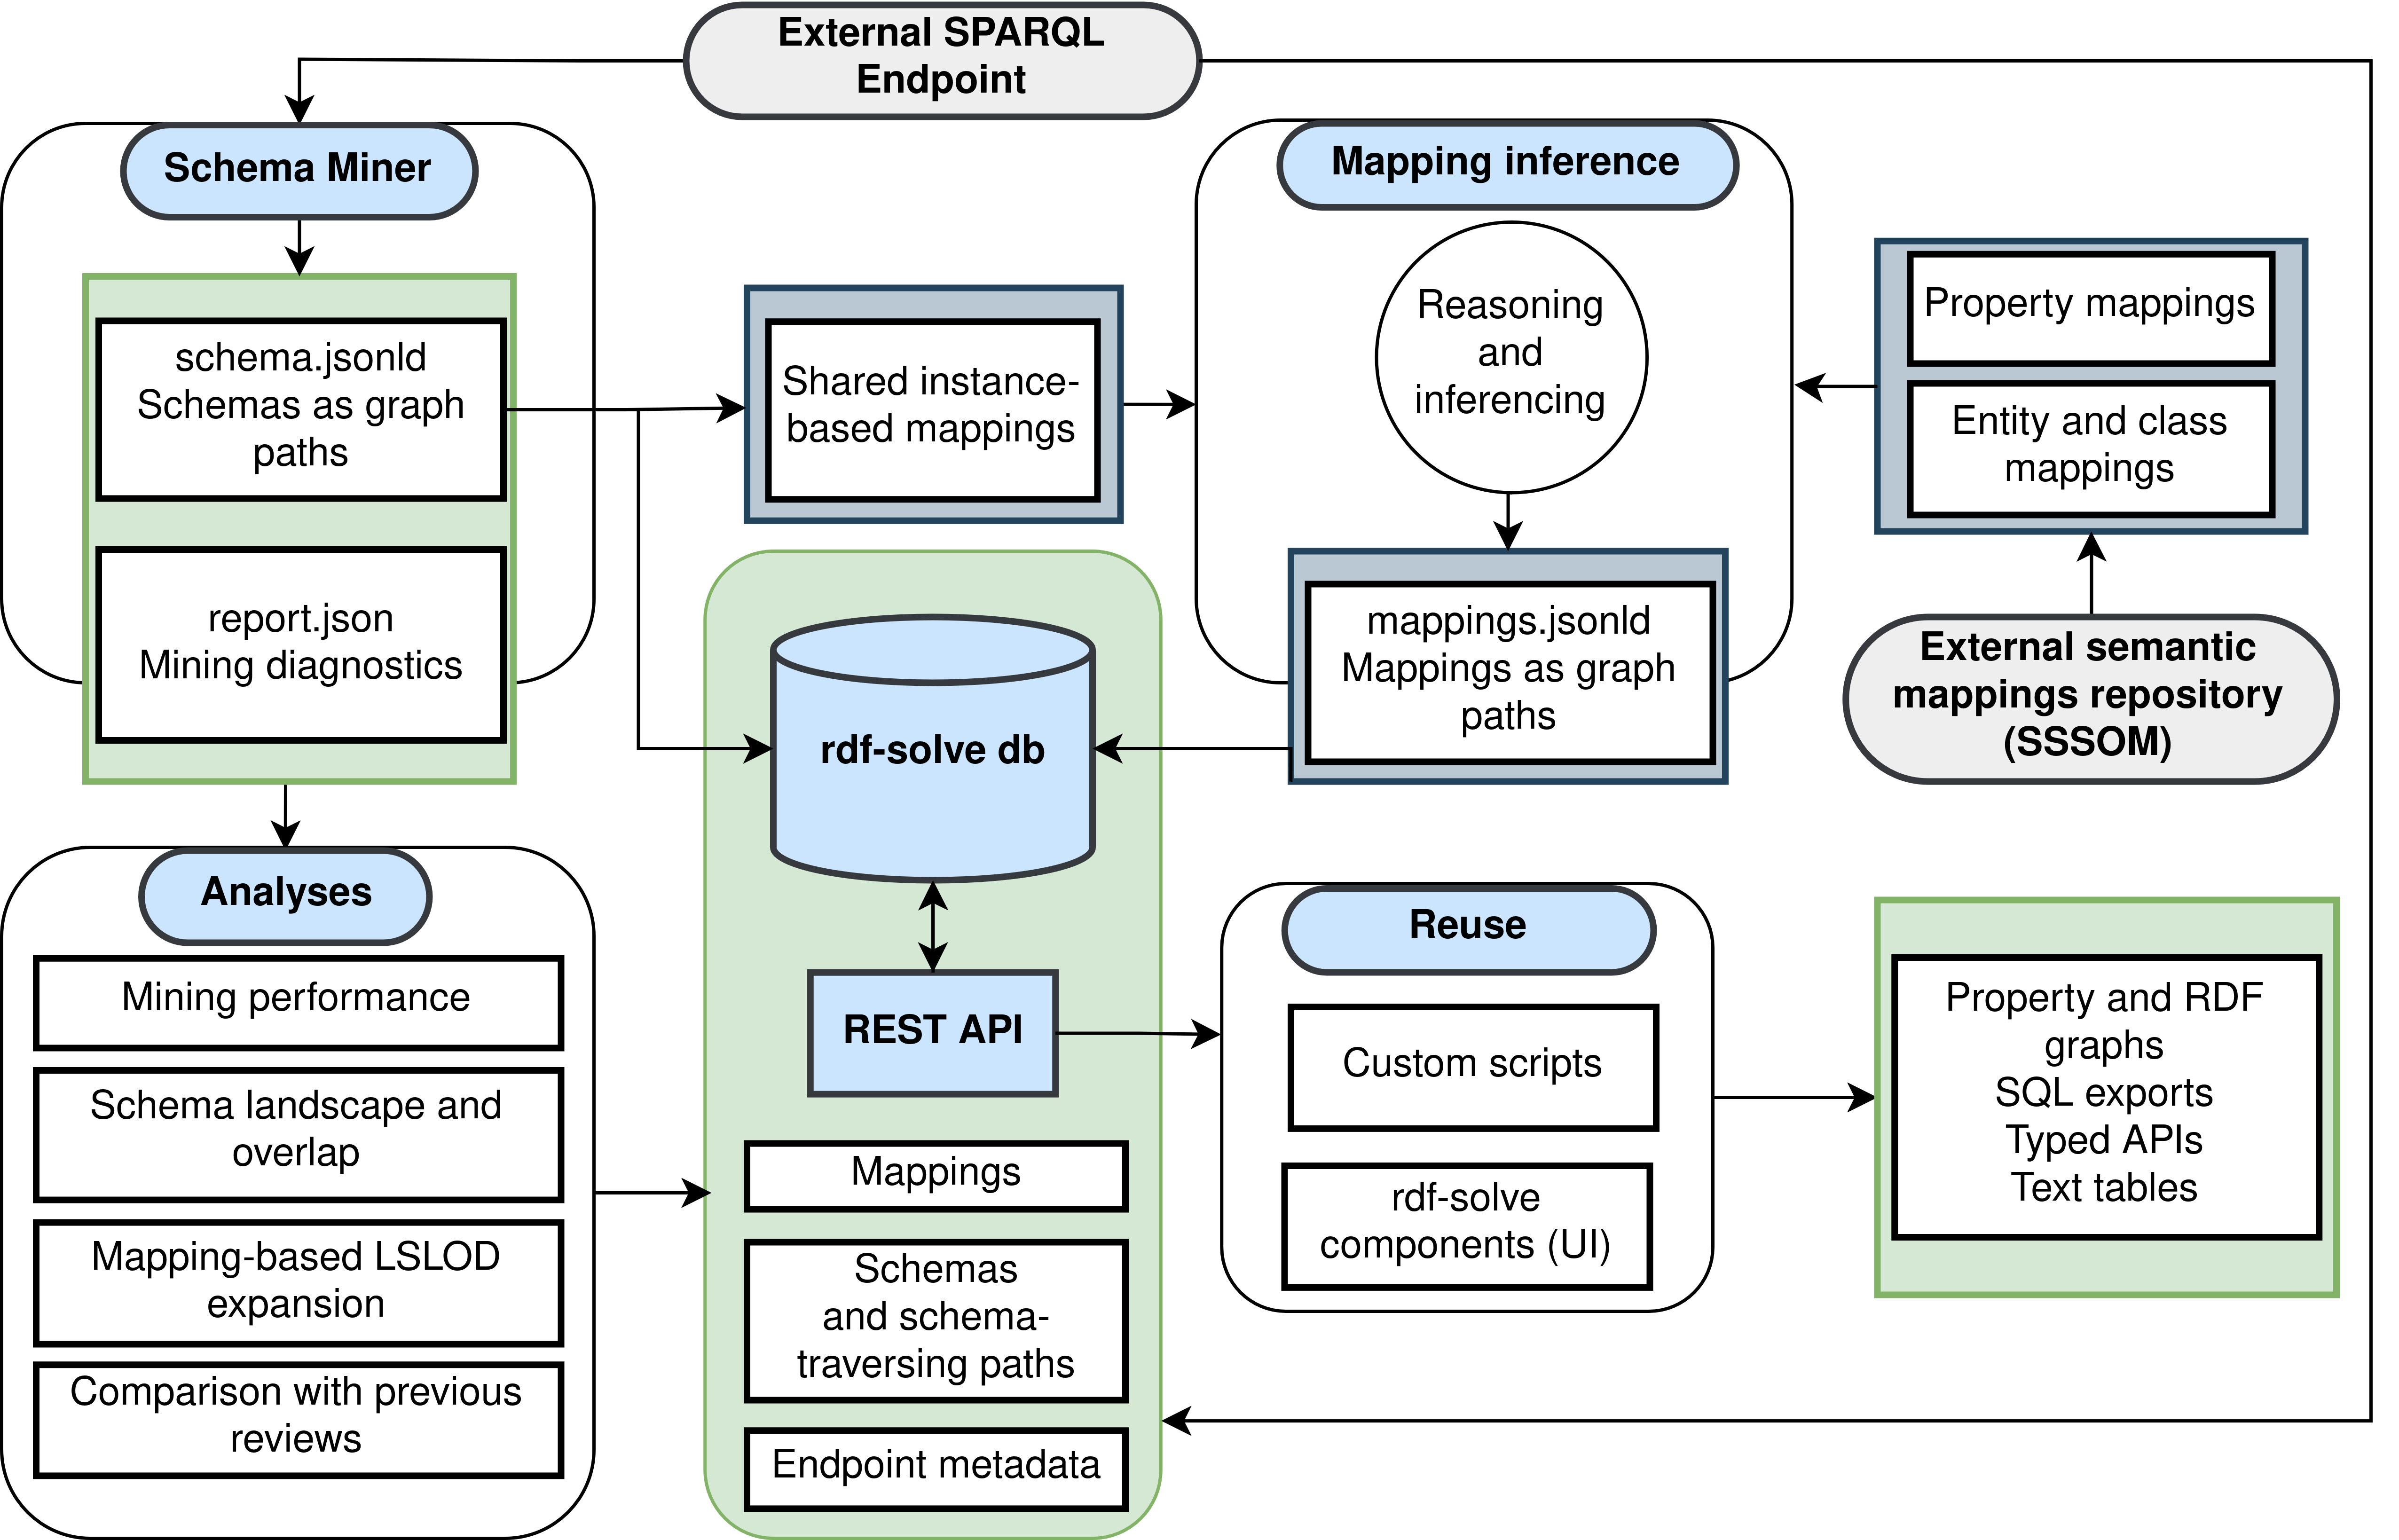
\includegraphics[width=1\linewidth]{figures/workflow.png}
\caption{Workflow for the rdf-solve (...)}
\label{fig:workflow}
\end{figure}

\subsection{Schema Mining}
\label{sec:mining}

rdf-solve approximates the schema of a SPARQL endpoint by mining
co-occurrence patterns from instance data.  The approach follows the
class-then-property extraction paradigm introduced by linked data
profiling tools~\cite{loupe2015,kamdar_empirical_2021} and used outside SPARQL
\cite{shexer} but extends it with three key differences: 
(i)~configurable class batching via
SPARQL \texttt{VALUES} bindings, reducing round-trips;
(ii)~a recursive fallback chain (bisection, pagination with adaptive
page sizing, and predicate-first decomposition) that degrades
gracefully instead of discarding classes on failure; and
(iii)~separation of pattern discovery from counting, ensuring that a
count-query failure does not lose already-discovered patterns.

Three pattern types are recorded: typed-object patterns $(c, p, o)$
where $o$ is the \texttt{rdf:type} of the object URI; literal
patterns $(c, p, \mathit{dt})$ where $\mathit{dt}$ is the object
datatype; and untyped-URI patterns $(c, p)$ where no
\texttt{rdf:type} was retrievable for the object under the current
graph scope and inference presented by the endpoint.

The treatment of the third pattern type is configurable.
In the default strategy, untyped-URI patterns are retained as bare
predicate links whose object type is unknown.
An alternative strategy promotes those object URIs to candidate
classes, effectively treating the absence of an explicit
\texttt{rdf:type} assertion as a modelling gap rather than an absence
of class membership.
Both strategies can be applied to the same indexed data in
consecutive passes, yielding two schema variants for the same source
that can be compared or combined.
This is particularly relevant for local mining (Section~\ref{sec:local-mining}),
where re-running the algorithm over an already-indexed QLever instance
adds negligible overhead.

Class and property labels are resolved from a priority-ordered label
vocabulary: \texttt{rdfs:label} is preferred, followed by
\texttt{skos:prefLabel}, \texttt{dc:title}, \texttt{IAO\_0000118}
(alternative term), and \texttt{skos:altLabel}.
This order reflects decreasing terminological precision: primary
semantic labels are preferred over bibliographic titles and curated
synonyms.
Falling back to the local URI fragment is a last resort.
The multi-vocabulary lookup is relevant for endpoints that use
OBO-style annotation properties rather than RDFS labels.

\paragraph*{Notation.}
$Q(B, G)$ denotes query template $Q$ evaluated for class batch $B$
restricted to the named graphs in $G$, a set of zero or more URIs
supplied via \texttt{--graph-uri}.
When $G = \varnothing$ no \texttt{GRAPH} clause is added and the
query runs over the endpoint's default dataset.
When $|G| = 1$ a single \texttt{GRAPH <uri> \{ \ldots \}} clause
wraps the pattern; when $|G| > 1$ a
\texttt{VALUES (?g) \{ \ldots \} GRAPH ?g \{ \ldots \}} block
iterates over each named graph.
In all cases the scope is a query-level restriction; endpoint dataset
configuration may override or ignore it.
$\top$ / $\bot$ denote success / failure (timeout or cost-limit).
$B_{[:m]}$ and $B_{[m:]}$ are the two halves of $B$ after splitting
at $m=\lfloor|B|/2\rfloor$; bisecting reduces the number of classes
in the \texttt{VALUES} binding, narrowing the class-filter scope and
isolating expensive classes into separate sub-queries.
$\ell_{\min}$: minimum page size (configurable via \texttt{--chunk-size})
below which pagination is abandoned.
$Q_C$: \texttt{SELECT DISTINCT ?c WHERE \{?s a ?c\}} (type
enumeration).
$Q_p(c)$: \texttt{SELECT DISTINCT ?p WHERE \{?s a <$c$>; ?p ?o\}}
(predicate enumeration for class $c$).
$Q_\mathrm{to}^p(c,p)$: $Q_\mathrm{to}$ restricted to predicate $p$
for class $c$.
$t \models (s,p,o)$: triple $t=(s',p',o')$ matches pattern $(s,p,o)$
operationally if the endpoint's evaluation of
\texttt{?s a <$s$>; <$p$> ?o; ?o a <$o$>} (or the literal/datatype
variant) binds $t$; this depends on the endpoint's graph scope,
asserted \texttt{rdf:type} triples, and any active inference regime.
$n_{(s,p,o)} = |\{t \mid t \models (s,p,o)\}|$ is the co-occurrence
count as returned by the endpoint's \texttt{COUNT(*)} aggregate.
$Q_\mathrm{to}^{cnt}$, $Q_\mathrm{lit}^{cnt}$,
$Q_\mathrm{uri}^{cnt}$: the corresponding
\texttt{SELECT \ldots COUNT(*) \ldots GROUP BY} variants of
$Q_\mathrm{to}$, $Q_\mathrm{lit}$, $Q_\mathrm{uri}$; they accept
the same \texttt{VALUES} batching and fallback chain.

\paragraph*{Procedure.}
\textsc{Query}$(B, Q, E, G)$ sends $Q(B, G)$ to endpoint $E$ as a
single \texttt{SELECT DISTINCT} query.
On $\top$ it returns the results immediately.
On $\bot$, if $|B| > 1$ the batch is bisected and each half retried
recursively: reducing the \texttt{VALUES} binding narrows the set of
classes evaluated per sub-query, so that a class whose query exceeds
the endpoint's cost limit does not cause the remaining classes in the
same batch to be skipped.
Pagination (\texttt{LIMIT}/\texttt{OFFSET}) is not tried for
multi-class batches because it may not reduce per-page cost on
endpoints that re-evaluate the full binding set for each page.
For single-class batches ($|B|=1$) the class filter is already
minimal, so the fallback is pagination (\texttt{LIMIT $\ell$} /
\texttt{OFFSET $k\ell$}, $k = 0, 1, 2, \ldots$).
If a page fails, $\ell$ is halved and that page is retried; if $\ell$
falls below $\ell_{\min}$ pagination is abandoned and, for
$Q_\mathrm{to}$, a predicate-first decomposition is attempted:
$Q_p(B[0])$ enumerates predicates $P$ and
$Q_\mathrm{to}^p(B[0],p)$ is called once per $p \in P$; if $Q_p$
itself fails, the class contributes no typed-object patterns.
Any results accumulated before pagination was abandoned are retained.
If all strategies fail, \textsc{Query} returns $\emptyset$.

Phase~1 enumerates the asserted instantiated types $C$ visible
under~$G$.
When a \texttt{class\_chunk\_size} is configured, queries are
paginated with (\texttt{LIMIT}/\texttt{OFFSET}) steps; otherwise $Q_C$ is sent
as a single unpaginated query.
In both cases the request is subject to the same bisect/paginate
fallback chain as Phase~2.
Phase~2 partitions $C$ into batches $B$ of configurable size and
calls \textsc{Query} three times per batch ($Q_\mathrm{to}$,
$Q_\mathrm{lit}$, and $Q_\mathrm{uri}$) accumulating patterns into
$S$.
If $G \neq \varnothing$ and Phase~2 yields $S = \emptyset$ despite
$C \neq \emptyset$, an \emph{ontology-graph fallback} is triggered:
Phase~2 is re-run with $G' = \varnothing$, because the named graph
may contain only class definitions while instances reside in the
default graph. % Example, when they have well-defined ontology vs data graphs, happens with SIB a lot
Optionally (enabled by default, disabled with \texttt{--no-counts}),
a counting phase follows: the unique subject classes in $S$ are
re-batched identically to Phase~2 and each batch is submitted as a
grouped \texttt{SELECT \ldots COUNT(*) \ldots GROUP BY} query through
\textsc{Query}, so count queries benefit from the same bisect and
pagination fallbacks as pattern queries.
If a count query fails for a particular class (after all fallbacks),
the corresponding patterns are retained in $S$ with no count.

\paragraph*{Execution strategy selection and schema completeness.}
For local QLever endpoints the preferred execution path is the one-shot
strategy: a single unpaginated \texttt{SELECT DISTINCT} issued before any
fallback is attempted.
If it succeeds, the schema is complete in one round-trip and the fallback
chain is never entered.
Only when the one-shot query fails does the pipeline activate the
multi-level fallback chain (Algorithm~\ref{alg:mine}).
Remote endpoints always begin with the fallback chain, as the endpoint's
timeout and cost-limit behaviour is unknown.

When a source has been mined under multiple execution strategies
(e.g.\ default and \texttt{untyped-as-classes}, or local and remote),
the pipeline selects the most complete result for downstream analysis.
Completeness is assessed by two criteria applied in order: first,
whether the counting phase succeeded for all classes (i.e.\ all patterns
carry co-occurrence counts rather than null); second, total pattern count.
The run with full count coverage is preferred; among runs with equal
coverage, the one with the larger pattern set is retained.
This selection is recorded in the provenance block of the emitted schema,
allowing the choice to be audited and overridden.

Algorithm~\ref{alg:mine} summarizes the full procedure.

\begin{algorithm}[H]
\caption{Schema pattern mining}
\label{alg:mine}
\begin{algorithmic}[1]
  \scriptsize
\Require endpoint $E$; graph scope $G$
\Ensure $S$ (observed co-occurrence patterns); $\emptyset$ for a
        batch may mean failure or genuinely no patterns;
        incompleteness is logged but not encoded in $S$
\State $S \leftarrow \emptyset$
\Statex
\textbf{Phase 1 — class discovery}
\State $C \leftarrow$ \Call{Query}{$\varnothing$, $Q_C$, $E$, $G$}
       \Comment{paginated if \texttt{class\_chunk\_size} set}
\Statex
\textbf{Phase 2 — pattern mining}
\For{each batch $B \subseteq C$}
  \State $S \leftarrow S \cup$ \Call{Query}{$B$, $Q_\mathrm{to}$, $E$, $G$}
         \Comment{typed-object patterns}
  \State $S \leftarrow S \cup$ \Call{Query}{$B$, $Q_\mathrm{lit}$, $E$, $G$}
         \Comment{literal patterns}
  \State $S \leftarrow S \cup$ \Call{Query}{$B$, $Q_\mathrm{uri}$, $E$, $G$}
         \Comment{untyped-URI patterns}
\EndFor
\If{$S = \emptyset$ \textbf{and} $C \neq \emptyset$ \textbf{and} $G \neq \varnothing$}
       \Comment{ontology-graph fallback}
  \State re-run Phase~2 with $G' = \varnothing$
\EndIf
\Statex
\textbf{Counting phase} (optional; skipped with \texttt{--no-counts})
\State $N \leftarrow \emptyset$
\For{each batch $B \subseteq C_S$}
        \Comment{$C_S$: unique subject classes in $S$}
  \State $N \leftarrow N \cup$ \Call{Query}{$B$, $Q_\mathrm{to}^{cnt}$, $E$, $G$}
         \Comment{typed-object counts}
  \State $N \leftarrow N \cup$ \Call{Query}{$B$, $Q_\mathrm{lit}^{cnt}$, $E$, $G$}
         \Comment{literal counts}
  \State $N \leftarrow N \cup$ \Call{Query}{$B$, $Q_\mathrm{uri}^{cnt}$, $E$, $G$}
         \Comment{untyped-URI counts}
\EndFor
\State $S \leftarrow \{\,(s,p,o,n_{(s,p,o)}) \mid (s,p,o)\in S\,\}$
        \Comment{merge; $n$ = \texttt{null} when no count retrieved}
\State \Return $S$
\Statex
\Function{Query}{$B$, $Q$, $E$, $G$}
  \If{$Q(B,G) = \top$} \Return results \EndIf
        \Comment{single \texttt{SELECT DISTINCT}}
  \If{$|B| > 1$} \Comment{bisect: isolates expensive classes into separate sub-queries}
    \State \Return \Call{Query}{$B_{[:m]}$, $Q$, $E$, $G$}
            $\cup$ \Call{Query}{$B_{[m:]}$, $Q$, $E$, $G$}
  \EndIf
  \State $R \leftarrow \emptyset$;\ $k \leftarrow 0$
  \Repeat \Comment{paginate single-class result set (\texttt{SELECT DISTINCT})}
    \If{page $Q(B,G,\ell,k) = \top$}
      \State $R \leftarrow R \cup \text{page results}$;\ $k \leftarrow k+1$
    \Else
      \State $\ell \leftarrow \ell / 2$;\ \textbf{retry page} $k$
      \If{$\ell < \ell_{\min}$} \textbf{goto} \textit{decompose} \EndIf
    \EndIf
  \Until{empty page received}
  \State \Return $R$
  \Statex
  \State \textit{decompose:}
  \If{$Q = Q_\mathrm{to}$} \Comment{predicate-first decomposition (last resort)}
    \State $P \leftarrow$ \Call{Query}{$\{B[0]\}$, $Q_p(B[0])$, $E$, $G$}
    \State \Return $\displaystyle\bigcup_{p \in P}$
            \Call{Query}{$\{B[0]\}$, $Q_\mathrm{to}^p(B[0],p)$, $E$, $G$}
  \EndIf
  \State \Return $\emptyset$ \Comment{strategies exhausted}
\EndFunction
\end{algorithmic}
\end{algorithm}

\subsection{Semantic mapping layer}

The mapping layer operates at four levels. Instance-based matching probes SPARQL endpoints
for bioregistry \cite{bioregistry} URI patterns to detect which datasets share entity
namespaces. This requires no prior knowledge of the schema and identifies candidate mapping
targets from the endpoint content directly. Curated mapping sets are imported via SSSOM sources,
adding support for frameworks like SeMRA \cite{hoyt_assembly_2025}, covering sources such as NCIT-ChEBI.
These are serialized as JSON-LD with one file per source-prefix pair. Inference then
propagates new links by applying transitivity, inversion, and evidence-chain composition
over the combined mapping graph as decribed in \cite{hoyt_assembly_2025}. 

The fourth layer maps predicates to allow relaxation of expressivity for semantically related 
predicates, allowing for link discovery and enabling property graph exports (THIS PART IS TODO).

All mappings carry provenance metadata including evidence chains and justification predicates 
from the SSSOM and semapv vocabularies.

\subsection{Integration of SPARQL examples}

TODO, get SHACL sparql executbales from endpoints or static sites and render their diagram.                                                                                   % I haven't written code for this yet: discover SPARQL executables and render their diagrams, etc.

\subsection{Query generator (web app)}
Querying, export queried data to (graph) databases, generate scripts to reproduce the steps in Python. TODO.    % Here, use property mappings to try to distille the simplest predicates to create e.g. neo4j exports. Mapping RO predicates to SIO predicates, then using more top-level options to not overfit, have a way to serialize that into documented Neo4j graphs, or use the LinkML exports to convert data + LinkML schema into SQL.

\subsection{Standard serializations}

Extracted schemas are serialized in several formats. JSON-LD documents include a provenance
block recording the extraction strategy, endpoint URL, generation timestamp, and pattern
count. This makes each schema self-describing and ready for downstream use without requiring
external metadata. VoID Turtle files describe class and property partitions following the
extended VoID vocabulary. SHACL shapes are generated from a LinkML intermediate and can be
applied directly for validation or repair. JSON-LD, SHACL and VoID turtles are compatible with
standard RDF tooling including rdflib and Apache Jena. The LinkML is also used for exports such
as pydantic Python APIs and SQL tables (work TODO).

Provenance blocks additionally record the tool version, Python version, 
duration, machine fingerprint, and, where supplied, the ORCID-bearing author list of the
person or workflow that triggered the extraction.
This allows mining runs to be cited and traced to specific pipeline invocations.
All schema and VoID artifacts are assigned canonical URIs under a shared base, so
cross-referencing between a report, its VoID catalog, and its LinkML schema is
machine-readable without extra configuration.

The web backend persists all artefact types (mined schemas, VoID catalogs, LinkML
schemas, and mining reports) in a structured store, and exposes them through
dedicated REST endpoints (\texttt{/api/reports}, \texttt{/api/void},
\texttt{/api/linkml}).
This decouples downstream consumers from the filesystem layout of the pipeline output
and allows artefacts to be queried, filtered by dataset or strategy, and downloaded
in their native formats (Turtle, YAML) directly via HTTP.

\subsection{Implementation and reproducibility}
\label{sec:implementation}

The methodology is packaged as two Docker images.

The \emph{pipeline container} bundles QLever, the format converters, and the
extraction and mapping tools; it is the environment used for all experiments
reported in this paper.
An orchestration script drives the complete workflow: building the image,
running remote discovery, generating per-source QLever configurations,
downloading and indexing each dataset, mining schemas locally, executing the
mapping and inference stages, and collecting results.
The script supports filtering to a subset of sources, skipping
already-completed stages, and optional machine-level benchmarking that records
wall time, CPU, and memory for each step.

A separate \emph{web application container} packages a Flask backend with a
SQLite store for the extracted schemas and mappings, together with a TypeScript
frontend for interactive exploration: dataset and mapping-source selection,
diagram-based schema visualization, a SHACL pattern browser and editor, and an IRI
resolver-based query generator.
The web container is not required to reproduce the results; it serves as an
interface for navigating the outputs produced by the pipeline.

\paragraph{Local mining}
\label{sec:local-mining}

Remote SPARQL mining depends on endpoint availability, rate limits, and timeout behavior,
all of which vary across engines and time. To decouple extraction from these constraints,
rdf-solve supports a local mining mode that operates on downloaded data dumps.

For each source that publishes downloadable data (N-Quads, RDF/XML, or compressed archives),
the pipeline generates a QLever configuration file containing the appropriate download and
conversion commands. QLever~\cite{bast_qlever_2017} indexes the data locally and exposes a
SPARQL endpoint, against which the same mining algorithm (Algorithm~\ref{alg:mining}) is applied.
QLever stores triples in six permutations with block-based compressed storage, enabling
efficient scans and joins over billion-triple graphs~\cite{bast_qlever_2017}; its
block-indexed \texttt{GROUP BY} and transitive property paths handle aggregation queries
that cause timeouts on other engines at scale~\cite{bast_sparqloscope_2025}.
Because the local engine runs without network overhead, timeouts, or rate limits, mining
completes faster and with fewer fallback activations.

The absence of network constraints makes a qualitatively different execution mode practical.
For local QLever instances the pipeline first issues a \emph{single unpaginated}
\texttt{SELECT DISTINCT} query that attempts to retrieve all typed-object patterns from the
full index in one request.  If this one-shot query succeeds, which it reliably does for
all but the very largest datasets, % This is what I think, wait to run the analyses in the server to re-write this
no fallback logic is needed and the schema is
complete in a single trip.  Only when the one-shot query fails (e.g.\ due to an
out-of-memory condition on an unusually large dataset) does the pipeline activate the
multi-level fallback chain described in Algorithm~\ref{alg:mining}: class-level bisection,
adaptive pagination, and predicate-first decomposition.
This execution path is \emph{only} available for local mining; remote endpoints always
begin directly with the fallback chain, since the endpoint's timeout
and rate-limit behaviour is unknown.

This local mode complements remote mining. Sources that offer both a SPARQL endpoint and
data dumps can be mined both ways, providing a cross-validation baseline for extraction
completeness. Sources with unstable or slow endpoints can be mined locally without depending
on their availability.

The pipeline supports executing the default and the untyped-as-classes extraction strategies
consecutively for each source without re-downloading or re-indexing.
The resulting pair of schema variants for each dataset allows downstream analysis to assess
how much additional structure is recovered when untyped URI patterns are promoted to classes,
and whether those candidate classes correspond to known ontology terms.

\section{Results}

\subsection{Mining performance and reliability}
\label{sec:results-mining}

We applied the mining algorithm (Section~\ref{sec:mining}) to $N$
SPARQL endpoints, including (...).

% what challenges depending on dataset? Some table based on report.json files

\paragraph*{Fallback utilization.}
For sources mined locally via QLever, the one-shot strategy succeeded in all cases tested,
with no fallback activations required. % Check this after running analyses, just a placeholder
Remote endpoint mining activated the fallback chain for a subset of sources where the
direct query timed out or returned partial results; the multi-level chain (bisection,
pagination, predicate-first) recovered the patterns in each case.
%some figure showing how many classes were recovered by each fallback strategy, and how many patterns were recovered by each strategy, to show the importance of fallbacks and the relative contribution of each one.

\paragraph*{Pipeline step timing.}
Figure~\ref{fig:pipeline-benchmarks} shows the duration of each pipeline step
recorded during a full run.  Total runtime includes either 
\begin{itemize}
\item{QLever indexing, one-shot schema
extraction, mapping import, inference expansion, and graph construction.
}
\item{
Remote endpoint mining, mapping import, inference expansion, and graph construction.
}
\end{itemize}
Depending on whether it was local or remote.
\begin{figure}[htbp]
  \centering
  % fig_pipeline_benchmarks.pdf/png generated by notebooks/mapping_analysis_paper.ipynb
  \IfFileExists{figures/fig_pipeline_benchmarks.pdf}{%
    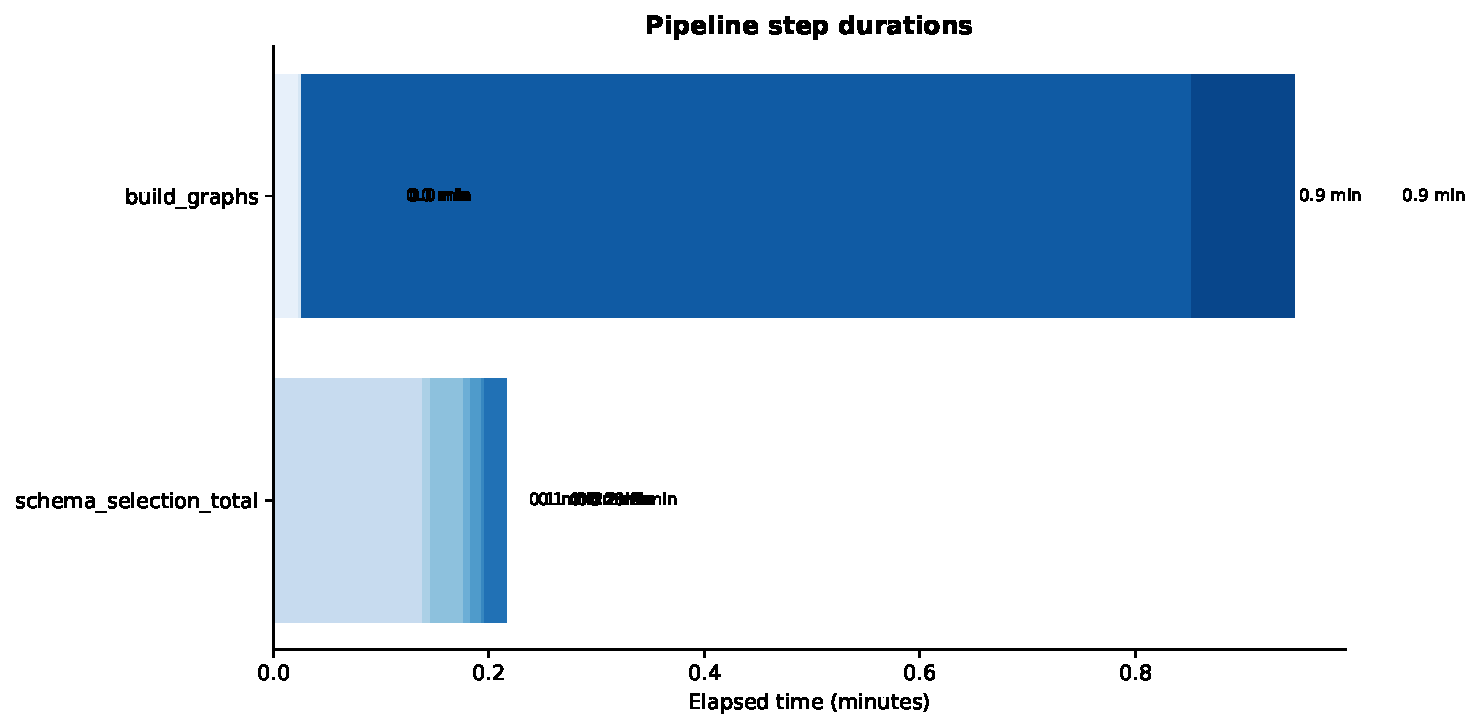
\includegraphics[width=\linewidth]{fig_pipeline_benchmarks}%
  }{%
    \fbox{\parbox{\linewidth}{\centering\itshape Figure placeholder: run
    \texttt{notebooks/mapping\_analysis\_paper.ipynb} to generate
    \texttt{figures/fig\_pipeline\_benchmarks.pdf}}}%
  }
  \caption{Duration of each pipeline step.
           Generated by \texttt{notebooks/mapping\_analysis\_paper.ipynb}.}
  \label{fig:pipeline-benchmarks}
\end{figure}

\subsection{Pattern coverage and structural profile}
\label{sec:results-patterns}

\paragraph*{Pattern-type distribution.}

\paragraph*{Class coverage.}

\begin{figure}[htbp]
  \centering
  % fig_schema_profile.pdf/png generated by notebooks/mapping_analysis_paper.ipynb  s13
  \IfFileExists{figures/fig_schema_profile.pdf}{%
    \includegraphics[width=\linewidth]{fig_schema_profile}%
  }{%
    \fbox{\parbox{\linewidth}{\centering\itshape Figure placeholder:
    \texttt{figures/fig\_schema\_profile.pdf}}}%
  }
  \caption{Distribution of pattern and class counts across mined schemas.
           Generated by \texttt{notebooks/mapping\_analysis\_paper.ipynb}.}
  \label{fig:schema-profile}
\end{figure}

\paragraph*{Property reuse across classes.}

\subsection{Mapping inventory and inference expansion}
\label{sec:results-mappings}

\paragraph*{Raw mappings.}
Instance matching identified which endpoint pairs share URI
namespaces, including Ensembl, UniProt, ChEBI, and FALDO identifiers.
%Some table of shared namespaces and counts.

\begin{figure}[htbp]
  \centering
  % fig_strategy_distribution.pdf/png generated by notebooks/mapping_analysis_paper.ipynb s5
  \IfFileExists{figures/fig_strategy_distribution.pdf}{%
    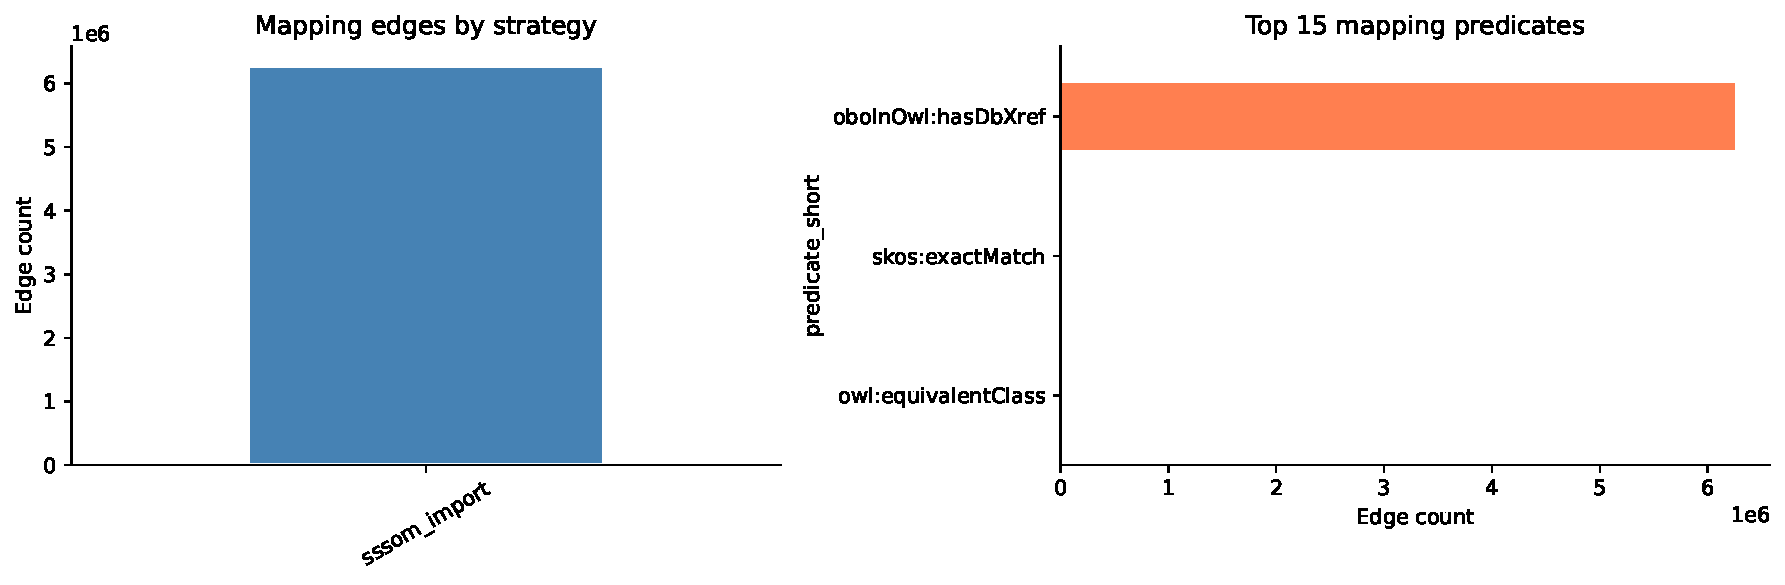
\includegraphics[width=\linewidth]{fig_strategy_distribution}%
  }{%
    \fbox{\parbox{\linewidth}{\centering\itshape Figure placeholder:
    \texttt{figures/fig\_strategy\_distribution.pdf}}}%
  }
  \caption{Distribution of mapping edges by strategy (left) and predicate (right).}
  \label{fig:strategy-dist}
\end{figure}

\paragraph*{Imported mappings.}
% For each SeMRA mapping set: number of mappings, prefixes covered,
% evidence types, how many classes could I resolve them to in the schemas

\paragraph*{Inference expansion.}
%some table or figure showing how many new mappings were inferred by each inference rule (transitivity, inversion, composition), and how many new endpoint pairs were connected by the inferred mappings.

\subsection{Cross-endpoint connectivity graph}
\label{sec:results-connectivity}

\paragraph*{Graph construction.}
% Nodes = datasets.  Edge (A,B) exists when a mapping edge (class_in_A, pred, class\_in\_B) has both classes present inthe respective mined schemas.
% Three variants: G_raw, G_inferred, G_schema.

\paragraph*{Connectivity metrics.}
% TABLE: for each graph variant — edges, connected components,
%        diameter, average degree, density.
Table~\ref{tab:graph_summary} summarises the connectivity of the three graph variants.
Each row corresponds to one variant; columns report node count, edge count, number of
connected components, largest-component size, diameter, graph density, number of Louvain
communities, and modularity.
% tables/tab_graph_summary.tex is generated by notebooks/mapping_analysis_paper.ipynb
% (Section 15 "Summary table"); run the notebook before compiling.
\IfFileExists{tables/tab_graph_summary.tex}{\begin{table}[h]
\caption{Summary of dataset-level graph properties and Louvain community structure.}
\label{tab:graph_summary}
\centering
\small
\begin{tabular}{l r r r r r r r r r}
\toprule
 & & & & $|V_{\text{lcc}}|$ & & & & & $|V_{\text{lcc}}|$ \\
Graph variant
 & $|V|$ & $|E|$ & $k$ & & $d$ & $\delta$ & $c$ & $Q$ & {\small comm.} \\
\midrule
$G_{\text{schema}}$   & 88 & 869 & 28 & 61 & 4 & 0.227 & 3 & 0.544 & 42 \\
$G_{\text{raw}}$      & 88 & 869 & 28 & 61 & 4 & 0.227 & -- & -- & -- \\
$G_{\text{inferred}}$ & 88 & 869 & 28 & 61 & 4 & 0.227 & 3 & 0.544 & 42 \\
\bottomrule
\multicolumn{10}{l}{\scriptsize $|V|$: nodes; $|E|$: edges; $k$: connected components;
$|V_{\text{lcc}}|$: largest component nodes;} \\
\multicolumn{10}{l}{\scriptsize $d$: diameter; $\delta$: density;
$c$: Louvain communities; $Q$: modularity; comm.: nodes in largest community.}
\end{tabular}
\end{table}
}{}

\paragraph*{Hidden bridges revealed by mappings.}
% Endpoint pairs reachable in G_inferred but not G_raw.
% These are connections revealed only by mapping inference.
% Report count and list representative examples.
Dataset pairs that are reachable in $G_{\mathrm{inferred}}$ but have no direct edge in
$G_{\mathrm{raw}}$ represent \emph{hidden bridges}: connections that exist only because
a transitive or inverse mapping chain links the two datasets indirectly.
Figure~\ref{fig:community-inferred} visualises how inference expansion reshapes the
community structure relative to Figure~\ref{fig:community-schema}.

\paragraph*{Hub ontology analysis.}
% For each class URI in mapping edges: how many datasets does it connect?
% Rank by betweenness centrality. 
Datasets with the highest betweenness centrality in $G_{\mathrm{inferred}}$ act as
integration hubs, bridging otherwise disconnected components.
The heatmap in Figure~\ref{fig:heatmap} shows the log-scaled edge weights for the
top datasets by betweenness centrality, highlighting the asymmetry between schema-level
and inference-expanded connectivity.

\paragraph*{Connectivity visualization.}

\begin{figure}[htbp]
  \centering
  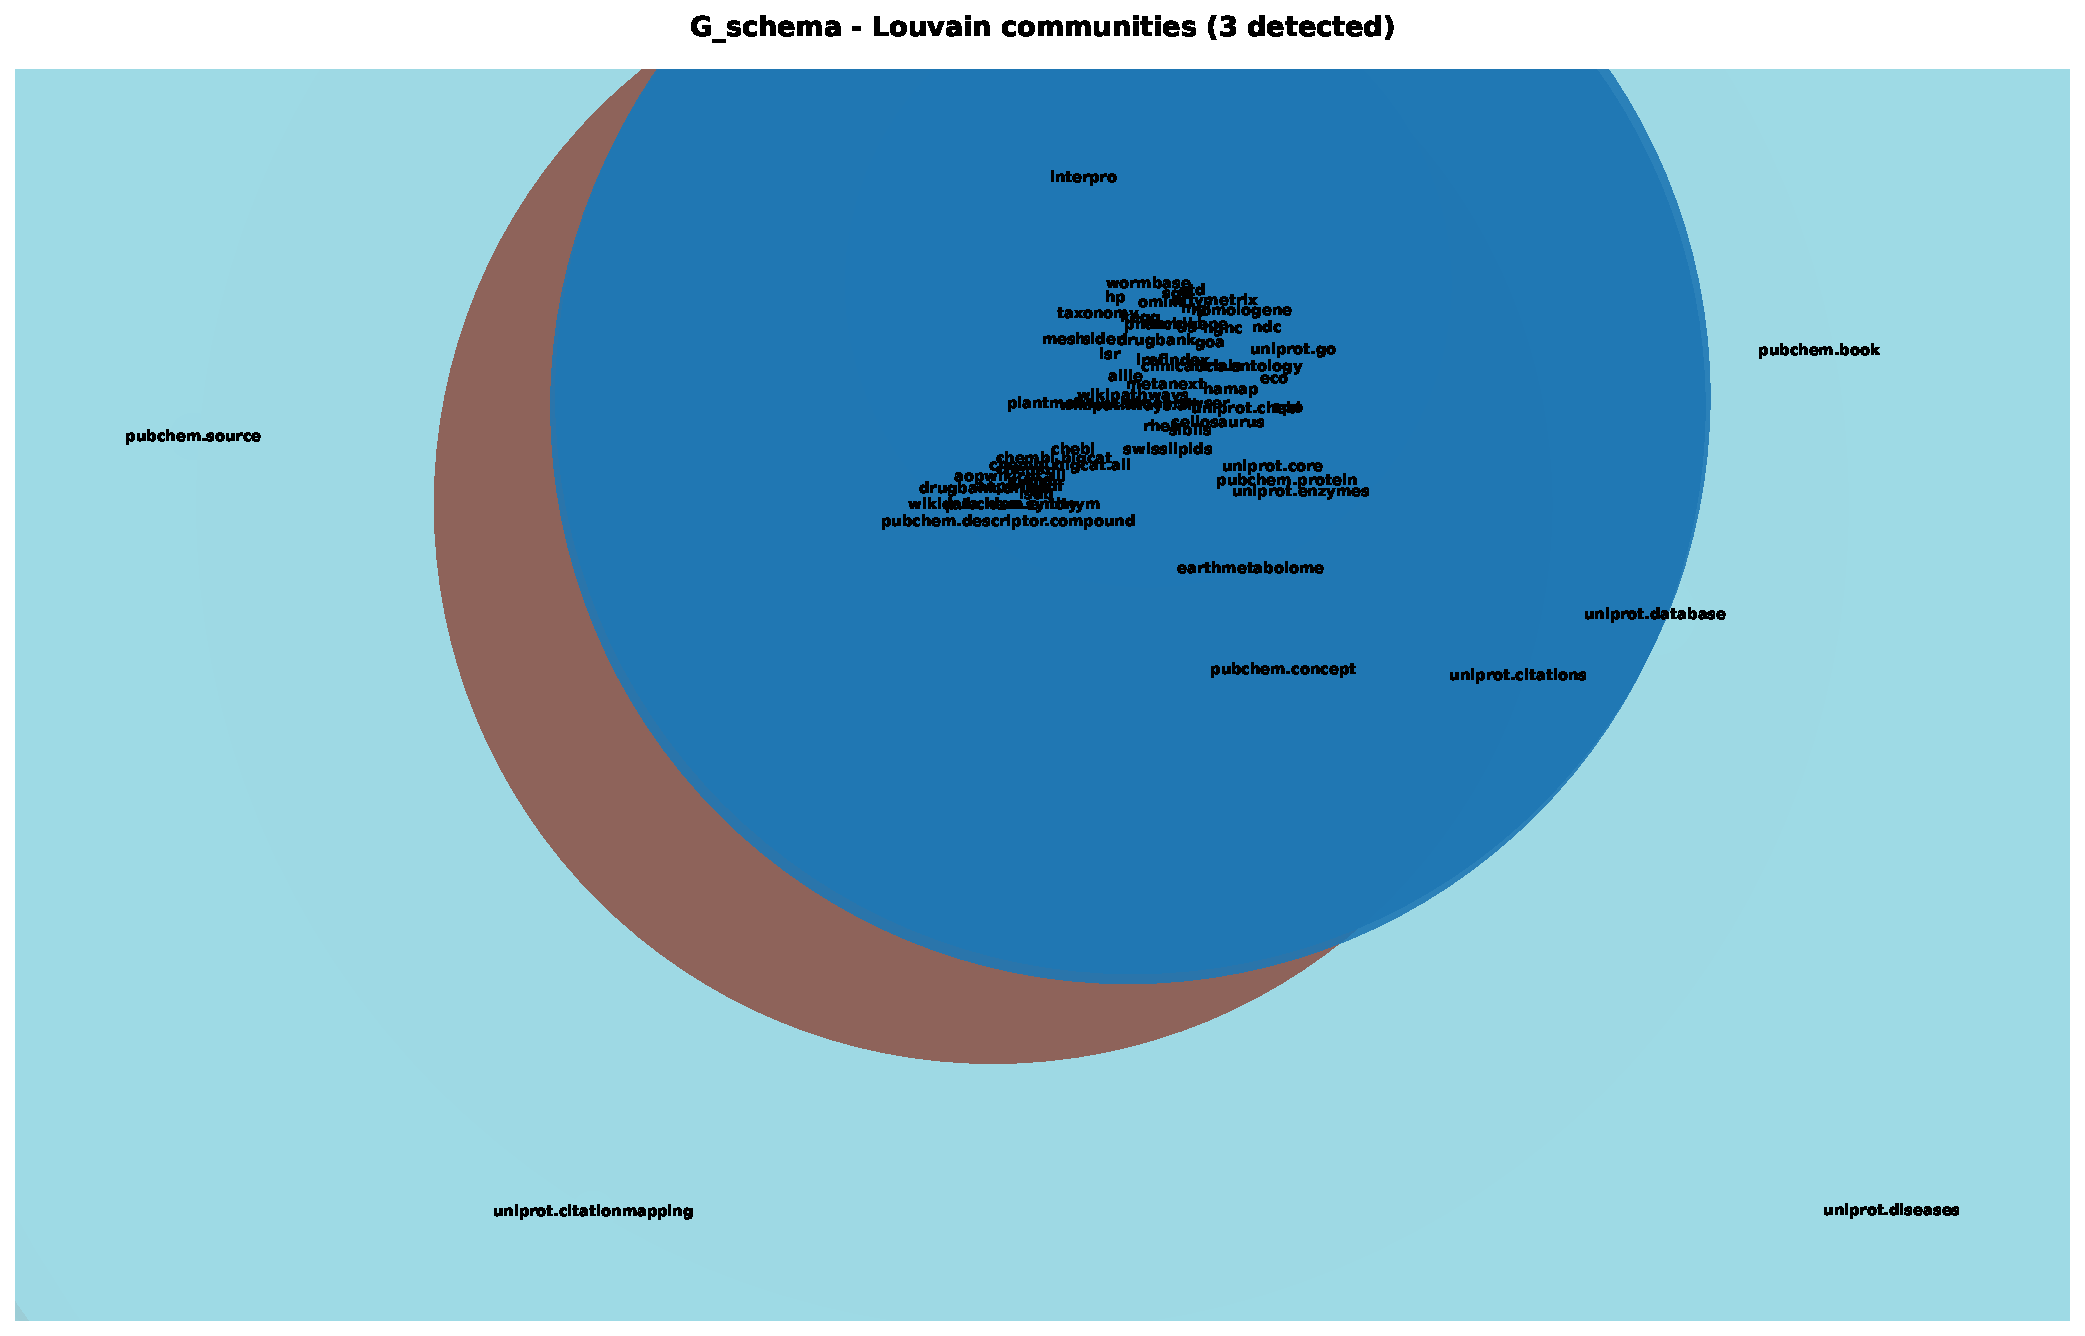
\includegraphics[width=\linewidth]{fig_community_gschema}
  \caption{Community structure of $G_{\mathrm{schema}}$.
           Nodes = datasets; edges = shared typed-object class pairs;
           colours = Louvain communities.}
  \label{fig:community-schema}
\end{figure}

\begin{figure}[htbp]
  \centering
  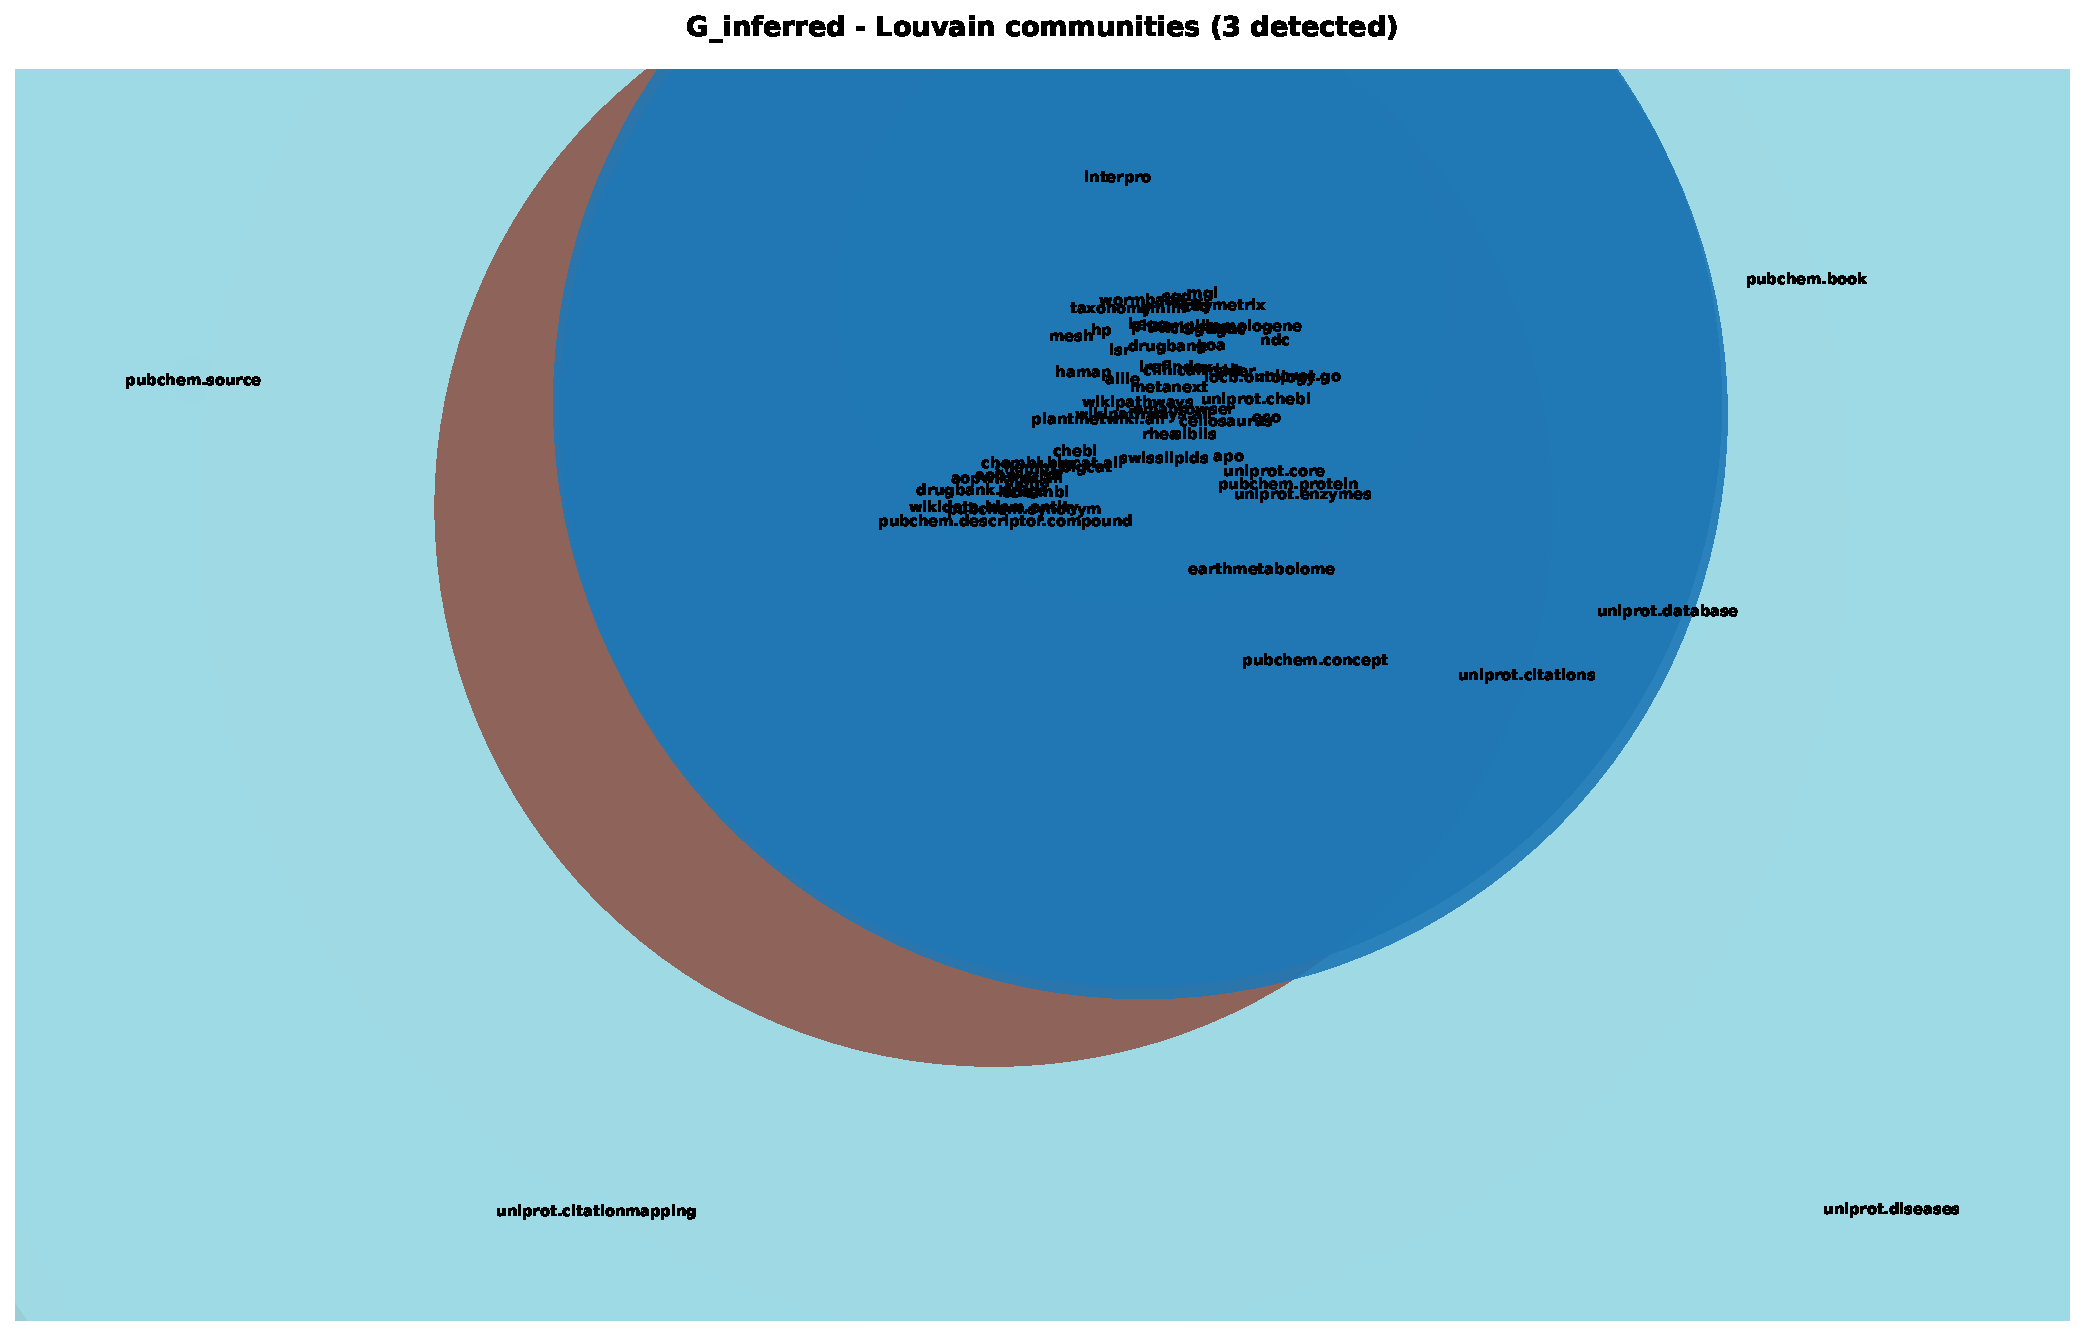
\includegraphics[width=\linewidth]{fig_community_ginferred}
  \caption{Community structure of $G_{\mathrm{inferred}}$ after all mapping
           layers and inference expansion.}
  \label{fig:community-inferred}
\end{figure}

\begin{figure}[htbp]
  \centering
  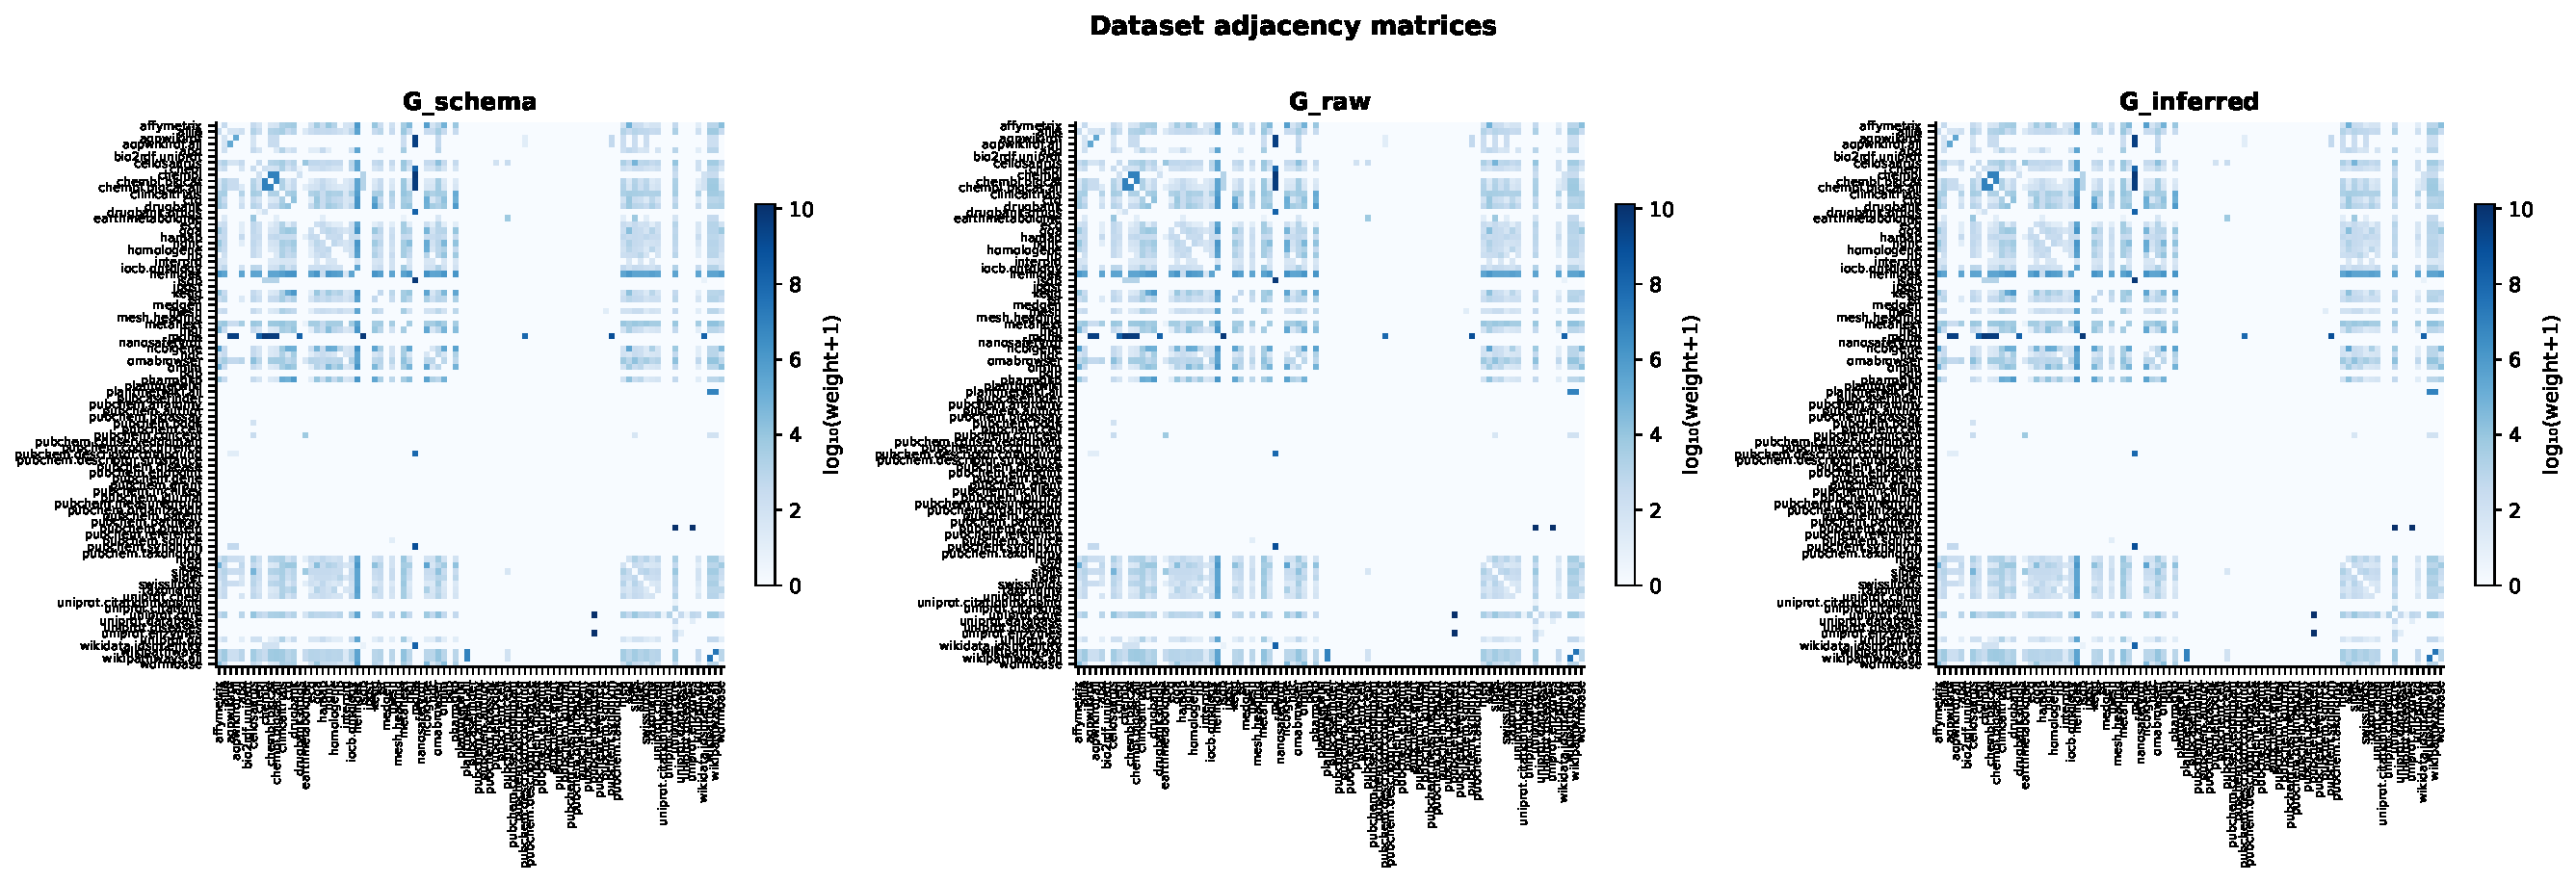
\includegraphics[width=\linewidth]{fig_heatmap}
  \caption{Log-scaled cross-dataset mapping weight for the top datasets by
           betweenness centrality in $G_{\mathrm{inferred}}$.}
  \label{fig:heatmap}
\end{figure}


\subsection{Case study: cross-endpoint traversal}
\label{sec:results-case-study}

% Pick ONE concrete traversal (e.g. Protein -> Pathway via UniProt -> WikiPathways through enzyme/protein class mapping).
% 1. Extract the traversal path from the connectivity graph.
% 2. Construct the federated SPARQL query using mined schemas + mappings.
% 3. Execute and show concrete result rows.
% 4. Estimate manual effort baseline: how long would it take a researcher to construct this query without rdf-solve?


\subsection{Comparison with prior work}
\label{sec:results-comparison}

% For overlapping endpoints with the previous meta-analysis paper: report schema evolution.
% Classes added/removed, properties changed.
% Attempt: longitudinal analysis of LSLOD schema drift, howvwer due to differences with the Kamdar methodology I doubt it will be any useful in practice, I need to see still but I assume from their SPARQL methods that they missed class patterns I could recover with my fallbacks. Also for counting, they just sampled 2000 entities so they likely missed stuff

\subparagraph*{Vocabulary reuse re-estimation.}
% Replicate Kamdar \& Musen Eq.~1 on our mined schemas using bioregistry (vs their BioPortal + LOV), we can also do BioPortal + LOV for direct comparison; find the reuse rate.
% Compare 2018 vs 2025 reuse rate however consider the differences in out mining methodologies at all times.

\paragraph*{Connectivity vs community detection.}
% Their communities answer which schema elements are similar, My connectivity graph answers "which databases can be joined?"

\subsection{Comparison with non-SPARQL-based mining methods}
% eg shexer


\subsection{Schema validation and refinement}
\label{sec:results-validation}

%% Something to say about using SHACL to "fix" a bigcat endpoint?

The methodology also exposes which classes are untyped in the RDF graphs (i.e., which RDF literals are used as classes by schemas), which
could be used iteratively to define new ontology classes need to be added in order for the endpoint to be self-documented.

\subsection{Traversal query generation and execution}
% This related to the rdfsolve typescript app

\section{Discussion}

\subsection{Work on title, why a tool on top of already powerful sparql engines}

Recent engineering work on QLever addresses the \emph{engine} side of
the scalability problem: block-based storage, precomputed predicate
patterns, and autocompletion over billion-triple
graphs~\cite{bast_qlever_2017,bast_autocompletion_2022}.
GRASP shows that an LLM agent can generate correct SPARQL for a
single, well-maintained endpoint by probing its schema
interactively~\cite{walter_grasp_2025}.
These are substantial technical advances.

\paragraph*{Cross-endpoint, not single-endpoint.}
QLever's autocompletion and GRASP's interactive probing address
queries against one endpoint.
Federated queries or dataset selection across the LSLOD cloud require
prior knowledge of which endpoints share compatible schemas.
The connectivity graph produced here provides that prior, though its
quality depends directly on the completeness of the mined schemas and
the precision of the imported mapping sets, both of which carry
known limitations (Section~\ref{sec:mining-discussion}).

\paragraph*{Persistent, citable artefacts versus on-the-fly discovery.}
GRASP discovers schema information at query time.
The artefacts produced here (VoID catalogs, SHACL shapes, LinkML
schemas) are static snapshots with provenance metadata.

\paragraph*{Open science outputs for under-resourced endpoints.}
The resources that QLever autocompletion and LLM approaches perform
best on tend to be large, consistently available, well-maintained
endpoints (Wikidata, UniProt).
Much of the LSLOD cloud is: small-to-medium databases
maintained by small groups, with intermittent support, no VoID-ext or other schema
descriptions, and no budget for infrastructure upgrades.
Publishing extracted schemas as linked data lowers the barrier for
tools and workflows that cannot query the source directly.
Whether this constitutes a meaningful contribution depends on adoption.

~\cite{kamdar_empirical_2021} concludes that the LSLOD
cloud "is not actually as densely connected as is often indicated",
with vocabulary reuse at under 20\,\% and many sources standing as
isolated RDF conversions.
Their community detection identified groups of semantically similar
schema elements across sources using word-embedding similarity,
revealing latent overlap invisible at the URI level. % But what didn't they do that I improve, and what exactly do I find, I can only write after running full analyses.
SynopsViz~\cite{bikakis_rdfsynopsviz_2014} and Sparklis~\cite{ferre_sparklis_2016} address
exploration and querying of individual sources but do not bridge the
gap across endpoints.
LODsyndesis provides connectivity metrics across hundreds of datasets
but operates on pre-computed indexes rather than live endpoint
mining.

We materialize the connectivity that prior analyses only
detected statistically.
The connectivity graph (Section~\ref{sec:results-connectivity}) identifies endpoint pairs
that can be concretely joined via shared ontology classes and inferred
mappings, answering ``which endpoints can be federated?'' rather than ``which schemas are similar?''

Curated mapping sets imported further cover cases where namespace alignment alone is insufficient. % When I have results I can quantify this or qualify it

\subsection{Provenance and reproducibility}

Each mining run produces a self-contained report that records the tool
version, extraction strategy, endpoint URL, graph scope, 
duration, warnings found, and the identity of the person or automated workflow that
triggered it.
These reports are assigned canonical URIs and cross-referenced with
their corresponding VoID catalog, LinkML schema, and SHACL shapes,
so the full provenance chain of any artefact can be reconstructed
without consulting external logs.

Documenting the extraction strategy, including
whether counts were collected and whether the untyped-as-classes
variant was applied, means that two schemas generated from the
same endpoint under different assumptions are distinguishable
in the record.
This is a prerequisite for any meaningful longitudinal comparison or
method benchmarking: conclusions about schema evolution or strategy
differences require that the methodological parameters of each run
are unambiguously captured alongside the results.

\subsection{Scalability and centralization}

Papadaki et~al.~\cite{papadaki} highlighted the difficulty of
achieving efficiency for complex aggregate queries at scale.

Kamdar and Musen~\cite{kamdar_empirical_2021} argued for centralized
top-down approaches to monitor accessibility and enforce vocabulary
reuse standards.

rdf-solve's multi-level fallback chain addresses the scalability
concern at the extraction level for external endpoints, recovering patterns for
queries tthat would otherwise fail under single-shot extraction.
The local mining pipeline (Section~\ref{sec:local-mining}) further
removes the dependency on remote endpoint availability entirely:
downloading data dumps and indexing them with QLever eliminates
network timeouts, rate limits, and engine-specific quirks from the
extraction path.
The containerized web application and batch-seeding scripts provide a
reusable infrastructure for periodic re-mining, moving toward the
centralized monitoring. % (...)

%Find more citations for this section, comparison.


\subsection{Mining robustness and the fallback contribution}

The multi-level fallback chain (bisect, paginate, predicate-first
decomposition) is an engineering contribution that enables all
downstream analyses. % I honestly believe this, I tried many approaches and often got too truncated/incomplete results

Prior remote endpoint miners, including the \cite{kamdar_empirical_2021} tool, use
single-shot queries per class and silently skip classes on timeout; Loupe~\cite{loupe2015}.  %carefully describe how Loupe does it
% TODO: cite fallback-utilization numbers from Section on mining results
% once available — expected: X\% of classes recovered only via bisection,
% Y\% only via pagination, Z\% via predicate-first decomposition.

The separation of pattern discovery from counting further ensures
that a count failure does not cascade into a pattern loss, a design
choice validated by the count-failure rate analysis.
% TODO: cite specific count-failure rates once results are available.

\subsection{Resulting LSLOD cloud}

\paragraph{Schemas}
\paragraph{Mapping layer}
% Expected discussion points:
% What results of mining schemas?

% - With 2020 Kamdar paper: Methodological: differences in mining strategy, does it mean differences in extracted classes cannot be attributed solely to schema evolution.
    % - How many of the original ~80 endpoints are still reachable?
    % - For overlapping endpoints: classes added/removed, properties changed.
    % - Vocabulary reuse re-estimation: replicate Kamdar Eq.1 on mined schemas using bioregistry (vs their BioPortal + LOV).
    % - Reference Kamdar data at https://doi.org/10.6084/m9.figshare.12402425

\subsection{Ontology reuse and matching}
% Expected discussion:
% - Make sure it is well defined
% - Quantify: for which endpoints does this occur, and how many "classes" are actually ontology leaf terms?
% - Possible mitigation: class-frequency thresholding, or post-mining clustering of classes that share identical property signatures.
% - Connect to Mihindukulasooriya: ontologies are designed for entailment, not validation, what will be this "meta-schema meta-ontology I produce? How can it be used?

\subsection{Mapping quality and evidence chains}

The mapping layer's quality is bound by its upstream sources.
Instance-based matching detects shared URI namespaces but does not
verify semantic equivalence; SeMRA-imported
mappings~\cite{hoyt_assembly_2025} inherit the precision and recall of their
curated sources.
Inference propagation (transitivity, inversion) amplifies both
signal and noise: transitive chains of length $\geq 3$ carry
multiplicative uncertainty.
The evidence-chain metadata preserved in the mapping JSON-LD
documents these provenance paths, but downstream consumers must
decide which evidence depth to trust.
% When I run analyses, attempt discussion:
% - Report mapping precision on a manually verified sample.
% - How many inferred mappings have chain length ≥ 3?
% - Does the connectivity graph change materially when filtering to high-confidence mappings only?
% - Connect to Kamdar's "intent for reuse": does instance matching actually resolve some of those cases, and which remain unresolved?

\subsection{Limitations of schema mining}
\label{sec:mining-discussion}



\paragraph*{Graph scope and invisible types.}
Phase~1 enumerates only types asserted via \texttt{rdf:type} and
visible under the chosen graph scope; inferred or unmaterialized
types are silently absent from $C$.
Graph selection is therefore a critical configuration choice.
The whole-endpoint mining variant (no named-graph restriction) with
post-mining service-namespace filtering addresses this partially:
it recovers patterns that would be missed under a strict graph scope,
at the cost of including infrastructure artefacts that must be
stripped.
% Expected: quantify how many additional classes the .all mining recovers
% vs named-graph-only mining, for endpoints where both are available.

\paragraph*{Remote mining.}
The remote mining step depends on endpoint availability, rate limits, and
engine-specific behavior, and is inherently liable to data incompleteness.
Failure risk for $Q_\mathrm{to}$ grows with instance count and object
cardinality, so the output may be biased toward small, well-indexed
classes.
When all fallback strategies fail, a batch contributes $\emptyset$ to
$S$, indistinguishable from a class with genuinely no patterns of
that type.
Failures are logged but cannot be encoded in $S$ itself.
% Expected: report how many classes hit the "strategies exhausted" path,
% and whether they are systematically the largest classes.

Different SPARQL engines (Virtuoso, Blazegraph, Fuseki, QLever)
exhibit different timeout behavior, error responses...
The fallback chain mitigates but does not eliminate these differences.
% Possibly a table of engine-specific quirks encountered during mining.

\subsection{Broader limitations and future work}

% discussion points for future expansion:

\paragraph*{Property-level mappings.}
Need more.



\paragraph*{Validation feedback loops.}
% After some manual inspection and changes, the SHACL shapes generated from mined schemas could be used to
%validate the source data itself, exposing quality issues that are invisible without a schema.
Feeding validation results back to dataset publishers would close the loop between schema mining and data
improvement~\cite{mihindukulasooriya_rdf_2018}.

\paragraph*{Downstream exports.}
LinkML intermediate representations open a path to SQL table
generation, property-graph exports (Neo4j), and typed Python APIs
(Pydantic). What else can be achieved?

\bibliographystyle{plain}
\bibliography{paper}

\end{document}
